\section{Problem Formulation and Leakage Taxonomy}\label{sec:problem}

\subsection{Task Definition}

We formalize fraud detection on ERP and payment data as per-transaction
binary classification over a temporal, directed, attributed multigraph. Let
$\mathcal{V}$ denote the set of entities (accounts, vendors, G/L codes, or
customers, depending on the dataset) and let
$\mathcal{D} = \{e_1, e_2, \dots, e_N\}$ denote the transaction set, where
each transaction is a tuple
\[
e_i = (u_i, v_i, t_i, a_i, \mathbf{c}_i, y_i),
\]
with origin $u_i \in \mathcal{V}$, destination $v_i \in \mathcal{V}$,
timestamp $t_i \in \mathbb{R}$ (or an ordinal step/day index --
Section~\ref{sec:datasets} details each dataset's time axis), amount
$a_i \in \mathbb{R}_{>0}$, an auxiliary attribute vector $\mathbf{c}_i$
(transaction/document type, channel), and a binary label
$y_i \in \{0,1\}$ recording confirmed fraud. Transactions induce a directed
multigraph $G = (\mathcal{V}, \mathcal{D})$ that grows monotonically in
time; we write
\[
G_{\le T} \;=\; \bigl(\mathcal{V},\, \{\, e_j \in \mathcal{D} : t_j \le T \,\}\bigr)
\]
for the graph state immediately after every transaction up to and
including time $T$ has posted. The task is to fit a scoring function
$f_\theta : \mathbb{R}^d \to [0,1]$, applied to a feature vector
$x_i = \phi(e_i, G)$ extracted for each transaction, that approximates
$\Pr(y_i = 1 \mid x_i)$. Three feature families compose $x_i$ in this
project: ordinary transaction attributes ($a_i$, $\mathbf{c}_i$, calendar
features), structural/topology statistics computed from the graph (degree,
fan-in/out, lapping recurrence, cycle membership), and, where used, learned
temporal-graph embeddings (TGN) \cite{rossi2020temporal}. The graph
neural network literature has repeatedly reported structure-aware models
outperforming tabular baselines on financial fraud tasks
\cite{motie2024gnn,yuan2025survey}, almost always without an explicit audit
of the temporal-leakage failure modes formalized below; the dataset roster
in Section~\ref{sec:datasets} is chosen so that a fair, leakage-controlled
version of that comparison is possible across a genuine range of
structural richness. With the class prior $\Pr(y=1)$ ranging from roughly
0.12\% to 1.21\% across the real datasets studied here
(Table~\ref{tab:datasets}), we follow standard practice for severely
imbalanced classification \cite{bishop2006pattern} and evaluate with
threshold-independent ranking metrics (PR-AUC / average precision,
precision@$k$) rather than accuracy or a fixed decision threshold; the full
metric discussion and the modeling protocol built on it are given later in
this paper.

\subsection{Leakage-Free Feature Computation}

The single methodological requirement that dominates every other design
decision in this project is that $\phi$ must not use information
unavailable at the instant $e_i$ posts. We state this precisely.

\begin{quote}
\textbf{Definition (leakage-free feature map).} A feature map $\phi$ is
\emph{leakage-free} with respect to $\mathcal{D}$ if, for every transaction
$e_i \in \mathcal{D}$,
\[
\phi(e_i, G) \;=\; \phi(e_i, G_{\le t_i})
\]
for any $G \supseteq G_{\le t_i}$ -- that is, $\phi$'s output for $e_i$ is
invariant to which transactions with $t_j > t_i$ are or are not present in
the graph.
\end{quote}

Operationally we enforce this with a single streaming pass over
$\mathcal{D}$ in non-decreasing timestamp order: for each $e_i$, (1)
\emph{read} $x_i = \phi(e_i, G_{<t_i})$ against the graph state already
committed, then (2) \emph{insert} $e_i$'s edge and any derived state
(running counts, expanding means, open cycle candidates) before moving to
$e_{i+1}$. This read-then-insert ordering makes look-ahead structurally
impossible rather than merely policy-forbidden -- no code path exists
through which a later transaction's data can reach an earlier
transaction's feature vector. Two corollaries follow directly and are
enforced throughout the engine: (a) no statistic used in a feature
computation -- mean, standard deviation, per-account baseline, Benford
digit distribution -- may be computed once over the whole dataset; every
such statistic must be expanding or rolling over the past only, and (b)
when a structure (a cycle, a lapping sequence) is only detectable once its
final edge posts, its signal attaches to that \emph{completing}
transaction, never retroactively to the earlier transactions that merely
participated in it. Train/validation/test partitioning follows the same
discipline: splits are chronological -- train on the earliest period,
validate on the next, test on the latest -- never a randomly shuffled
$k$-fold, a protocol documented elsewhere to silently leak the future into
the past on time-evolving, dynamic fraud data \cite{jesus2022turning}.

\subsection{Leakage Taxonomy: Two Failure Modes in the Predecessor System}

An earlier iteration of this codebase reported headline metrics as strong
as $\mathrm{ROC\text{-}AUC} \approx 0.997$ on its flagship dataset and
concluded that graph topology was fraud detection's ``ultimate
differentiator.'' A pre-registration audit of that system's own artifacts
found the opposite: its topology detectors scored essentially 0.0 feature
importance, and every reported number was contaminated by two independent,
stacked leakage mechanisms. We name them Leak Class A and Leak Class B and
treat their elimination as this project's primary internal-validity
requirement.

\textbf{Leak Class A -- whole-graph feature computation.} The predecessor's
topology detectors ran once over the \emph{entire} graph, with no
$t_j \le t_i$ restriction anywhere, and each detected structure's signal
was written back to every member transaction, including its earliest ones
-- a cycle only observable once closed was nonetheless flagged on the edge
that opened it, directly violating the definition above. Two concrete
symptoms make the violation unambiguous: (i) a feature literally named
\texttt{time\_to\_next} -- the number of seconds until each account's
\emph{next} transaction -- ranked among the top five features by
importance; no detector can know the gap to a future transaction without
having already observed it. (ii) Every z-score / anomaly feature was
standardized against a whole-dataset mean and variance computed once, so a
transaction dated on day one was scored against a ``normal'' baseline that
included transactions from every later day, test period included.

\textbf{Leak Class B -- modeling-protocol leakage.} Four compounding,
confirmed malpractices were present in all five of the predecessor's
training scripts. (i) SMOTE oversampling and class-weighting were applied
\emph{simultaneously}, double-correcting for imbalance; because SMOTE's
$k$-nearest-neighbor interpolation was applied indiscriminately to
topology columns, it manufactured physically impossible points (a
synthetic transaction with, e.g., 0.4 of a closed cycle) that eased the
learned boundary without corresponding to any real fraud pattern. (ii)
Every reported metric used the library's default 0.5 decision threshold
(\texttt{.predict()}), never a threshold selected on held-out data --
meaningless when the positive class is 0.1--1.2\% of rows, since 0.5 is
not an operating point anyone chose. (iii) Cross-validation used
\texttt{StratifiedKFold} with shuffling and the timestamp column dropped
before fitting, so folds routinely trained on transactions dated after the
ones being scored, layering random-future leakage directly on top of Leak
A. (iv) Models were selected by F1 at that same fixed 0.5 threshold rather
than a threshold-independent, imbalance-appropriate ranking metric, which
rewards whichever leak-inflated configuration happens to look best at an
arbitrary cutoff rather than the one that generalizes.

\textbf{Why each invalidates the reported numbers.} Leak A inflates
apparent predictive power because the model is not learning what is
knowable at the moment an investigator would act -- it is learning the
correlation between a label and events that, by construction, occur after
the label's determining moment; the resulting metric is not an estimate of
deployable detection ability at all. Leak B compounds this at the
evaluation layer: synthetic minority points generated from a distribution
informed by the whole, undifferentiated dataset bias the decision boundary
toward the very examples later used to measure it; shuffled folds directly
violate the temporal ordering a fraud investigation depends on; and
selecting the ``best'' configuration by a metric computed under both prior
leaks means every design choice in the pipeline was made with implicit
knowledge of the answer it would later be graded on. Under datasets this
imbalanced -- as few as 19--25 confirmed fraud transactions in a single
evaluation split for SAP W\"urzburg (Section~\ref{sec:datasets}) -- even a
handful of leaked examples can move a headline metric by tens of points,
which is precisely the failure mode the leakage-free construction above,
and the ablation protocol built on it, are designed to make structurally
impossible rather than merely audited for after the fact.

%% FIGURE TODO: two-track timeline diagram. Top track: the correct
%% read-then-insert order -- for a transaction at time T, an arrow reads
%% features from graph state at T (pointing only left/backward in time),
%% then a second arrow commits/inserts the edge, moving strictly
%% left-to-right with no arrow ever pointing forward. Bottom track: the
%% predecessor system's Leak A pattern -- a completed-cycle icon at day 40
%% sends an arrow backward past day 40 to overwrite/attach to feature
%% values at day 3, visually contrasting causal vs. acausal attribution of
%% the same structure.
\begin{figure}[t]
  \centering
  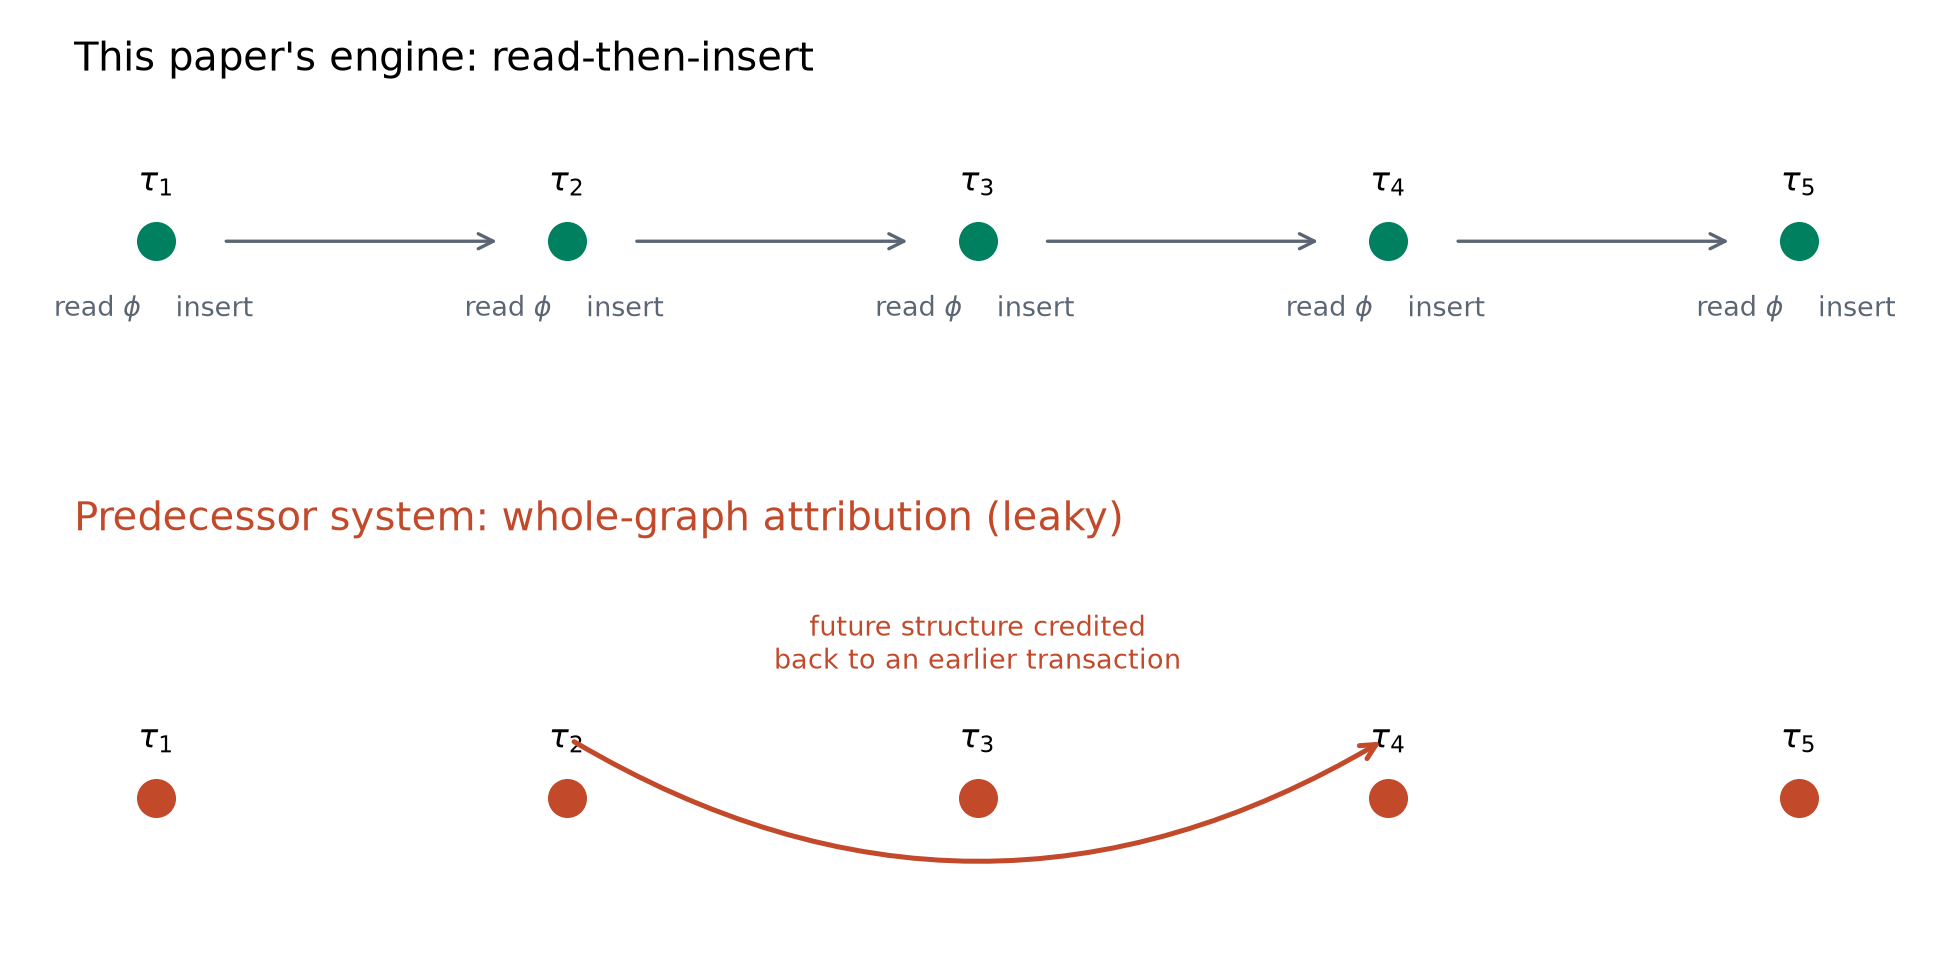
\includegraphics[width=\columnwidth]{figures/leakage_timeline.png}
  \caption{Read-then-insert feature computation (top) versus the
  predecessor system's whole-graph attribution (bottom), which credited a
  structure's signal back to transactions that occurred before the
  structure existed.}
  \label{fig:leakage_timeline}
\end{figure}

\section{Datasets}\label{sec:datasets}

\subsection{Overview and the Topology-Richness Spectrum}

Because the hypothesis under test is whether \emph{graph structure} carries
predictive signal beyond a strong tabular baseline, the dataset roster is
presented here as points along a topology-richness spectrum rather than as
an arbitrary convenience sample: from IBM AML, whose sender and receiver
identifiers occupy a near-unified account namespace supporting true
multi-hop cycles, down to PaySim, whose transaction graph is a near-forest
of one-off pairs. Table~\ref{tab:datasets} summarizes the four datasets
computationally profiled end-to-end in this study -- IBM AML, BankSim, SAP
W\"urzburg, and PaySim -- drawn from a single calibration pass over each
dataset's fully processed transaction table
(\texttt{calibration\_reference.json})
\cite{altman2023realistic,lopezrojas2014banksim,lopezrojas2016paysim}.
\emph{Kind} records each dataset's native graph topology: \texttt{Transfer}
(a directed account$\to$account graph, as in a payments network),
\texttt{Bipartite} (two structurally disjoint node classes with no
possibility of reciprocation or cycles), or \texttt{ERP ledger} (the
document-to-ledger-account bipartite structure specific to double-entry
ERP postings). \emph{NS Overlap} is the fraction of an account
namespace's senders that also appear as receivers -- the diagnostic this
project uses to certify whether same-entity cycles are even structurally
detectable; the predecessor system failed exactly this check by splitting
senders and receivers into disjoint node types, making a loop
$A\to B\to A$ structurally invisible regardless of how good its topology
engine was. \emph{Reciprocity} is the fraction of unique
(sender, receiver) pairs for which the reverse pair also transacted. Of
the four datasets in Table~\ref{tab:datasets}, only PaySim was profiled
without being modeled (Section~\ref{sec:paysim}).

\begin{table}[t]
\centering
\small
\caption{Graph-topology and scale summary of the four real datasets
computationally profiled in this study (source:
\texttt{calibration\_reference.json}). Amounts are in each dataset's
native units and are not comparable across datasets.}
\label{tab:datasets}
\resizebox{\columnwidth}{!}{%
\begin{tabular}{lccccccccc}
\toprule
Dataset & Kind & Fraud \% & $N_{\text{fraud}}$ & $N_{\text{txn}}$ & $N_{\text{acct}}$ & Amt.\ Med. & Benford MAD & NS Overlap & Recip. \\
\midrule
IBM AML       & Transfer    & 0.130 & 1{,}719 & 1{,}323{,}234 & 9{,}999       & 156.71      & 0.0758 & 0.9927 & 0.0446 \\
BankSim       & Bipartite   & 1.211 & 7{,}200 & 594{,}643     & 4{,}162       & 26.90       & 0.0319 & 0.0000 & 0.0000 \\
SAP W\"urzburg & ERP ledger & 0.124 & 248     & 200{,}629     & 59{,}883      & 1{,}975.80  & 0.0385 & 0.0000 & 0.0000 \\
PaySim        & Transfer    & 0.129 & 8{,}213 & 6{,}362{,}620 & 9{,}073{,}900 & 74{,}871.94 & 0.0142 & 0.0002 & 0.0000 \\
\bottomrule
\end{tabular}%
}
\end{table}

\subsection{IBM AML}

IBM AML is generated by the AMLSim multi-agent simulator and released as a
synthetic-but-structurally-realistic anti-money-laundering benchmark
\cite{altman2023realistic}. Its 1{,}323{,}234 transactions connect 9{,}999
accounts with a sender/receiver namespace overlap of 99.27\% -- the same
account IDs act as both senders and receivers almost everywhere, the
pre-condition this project treats as necessary for account-to-account
cycle detection to be structurally possible at all. Every transaction
carries the type \texttt{TRANSFER}; time is an integer day index over a
199-day span. At a fraud rate of 0.130\% (1{,}719 of 1{,}323{,}234), IBM
AML is this project's richest-structure testbed and the dataset on which
the topology hypothesis is given its best chance to succeed. It also
exhibits the sharpest amount anomaly of any dataset studied: fraud amounts
have median 10.60 and mean 9.76, against a full-population median of
156.71 and a mean of 115{,}988.18 (99th percentile 1{,}854{,}724.69) --
fraud in IBM AML clusters in a narrow, near-zero-value band while the
legitimate population is heavily right-skewed toward large transfers. We
read this as an artifact of the AMLSim generator's labeling convention
rather than a general property of laundering behavior, and it materially
shapes the ablation results discussed later in this paper: an
amount-based baseline that expects fraud to look large is directionally
wrong on this dataset, which is exactly what motivates evaluating an
amount-blind probe to isolate topology's contribution independent of this
artifact.

\subsection{BankSim}

BankSim is an agent-based simulation of a bank payment network built
specifically for fraud-detection research \cite{lopezrojas2014banksim}.
Its 594{,}643 transactions connect customer accounts (prefix \texttt{C})
to merchant accounts (prefix \texttt{M}) -- two structurally disjoint node
classes, so namespace overlap and pair reciprocity are both exactly 0.0
and no customer-to-customer or merchant-to-merchant cycle can exist by
construction. BankSim therefore serves this study as the sparse control:
any predictive lift topology features provide here must come from
bipartite-graph statistics (degree, fan-in/out, recurring near-equal
``lapping'' amounts) rather than from cycles, since cycles are
structurally unavailable. Its fraud rate, 1.211\% (7{,}200 of 594{,}643),
is the highest of the four real datasets, and its amounts are the smallest
in scale (median 26.90).

\subsection{SAP W\"urzburg}

SAP W\"urzburg is a real, publicly released SAP ERP transaction ledger and
is the only dataset in this study drawn from an actual production
accounting system rather than a simulator -- the setting continuous-
auditing research argues automated, always-on control monitoring should
target \cite{vasarhelyi2012acceptance}, and one that broader ERP-analytics
surveys still treat as an emerging rather than mature application of
machine learning \cite{jawad2024erp,mamakou2024postimplementation}. Its
graph is a document-to-account bipartite structure native to double-entry
bookkeeping: each posting document fans out to a small number of line
items (out-degree median 2.0, 99th percentile 10.0) that land on accounts,
a minority of which absorb a disproportionate share of postings (in-degree
99th percentile 43{,}706.7, maximum 46{,}554, against 59{,}883 distinct
account identifiers in total) -- a small core of heavily used ledger
accounts against a long tail of low-traffic counterparty accounts. With
only 248 confirmed frauds among 200{,}629 postings (0.124\%), SAP
W\"urzburg is this project's thinnest fraud signal by count, and, as the
ablation study reported later in this paper shows in full, the one real
dataset on which the full-model topology lift is measured
\emph{negative}. Two different SAP W\"urzburg train/validation/test
partitions appear elsewhere in this paper and should not be confused: the
chronological, partition-aware split used in the within-dataset ablation
study yields 120{,}411/40{,}137/40{,}139 rows
(\texttt{ablation.json}), while the multi-seed split used for final
champion-model selection yields 120{,}341/40{,}114/40{,}116 rows on the
same source file under a different, non-partition-aware split procedure
(\texttt{final\_champions.json}); both carry the same fraud counts by
split (204/19/25). We flag the discrepancy here so it does not appear
silently across two disconnected tables.

\subsection{IBM AML: Kaggle Reproduction Variant}

A second, independently downloaded instance of the IBM AML benchmark --
sourced directly from its Kaggle mirror rather than from the AMLSim-format
repository export behind the headline IBM AML numbers above -- was
processed during this build as a reproduction check on the deployed
\emph{online} scoring bundle, never as a source of headline results. The
two sources use different raw schemas (\texttt{TX\_ID}/
\texttt{SENDER\_ACCOUNT\_ID}-style AMLSim export versus the Kaggle
\texttt{HI-Small\_Trans.csv} layout) and are, in general, different
simulator draws; we report results under the separate label
\texttt{ibm\_aml\_kaggle} throughout, and none of its numbers are merged
into or averaged with \texttt{ibm\_aml}'s. For contrast -- though the two
are not directly comparable -- the offline champion model trained on the
primary \texttt{ibm\_aml} source, which includes TGN embeddings and, since
its TGN memory state is never persisted to disk, is not servable online at
all (a limitation discussed in full elsewhere in this paper), reaches a
saturated test PR-AUC of 1.00; that ceiling is itself uninformative given
the baseline's own 0.990 saturation (also discussed later in this paper).
\texttt{ibm\_aml\_kaggle}'s \emph{online} (ordinary+topology, non-TGN)
bundle -- the only kind of bundle this project ever serves in production
(\texttt{online\_bundles.json}) -- reaches a materially lower test PR-AUC
of 0.512 ($\pm$0.067 over three seeds, 26 features), consistent with both
the missing TGN component and the fact that the two \texttt{ibm\_aml}
variants are different simulator draws, not repeated measurements of the
same result.

\subsection{PaySim: Profiled, Not Modeled}\label{sec:paysim}

PaySim simulates a mobile-money transfer network at substantially larger
scale than any other dataset in this study -- 6{,}362{,}620 transactions
over 9{,}073{,}900 accounts \cite{lopezrojas2016paysim}, where almost
every transaction is the only time its particular (sender, receiver) pair
ever transacts (namespace overlap 0.0002, zero pair reciprocity, zero
repeat-pair transaction fraction). Its fraud rate, 0.129\% (8{,}213 of
6{,}362{,}620), sits in the same narrow band as IBM AML and SAP
W\"urzburg, but its graph is a near-forest at the opposite end of the
topology-richness spectrum from IBM AML: with essentially no repeated
edges between the same two accounts, most multi-hop structural detectors
(cycles, recurring lapping, degree accumulation) have little to attach to
before a transaction resolves. Consistent with this project's tiered
dataset plan, PaySim was carried through the ETL and topology-profiling
stages reported in Table~\ref{tab:datasets} but was never carried into
model training or the ablation study reported later in this paper; no
PR-AUC, precision@$k$, or lift number exists for it anywhere in this work,
and its row in Table~\ref{tab:datasets} should be read purely as a
structural reference point completing the spectrum, not as a modeling
result.

\subsection{The Synthetic Economy: synth\_erp}

\texttt{synth\_erp} is this project's own agent-based synthetic ERP
economy, spanning 39{,}256 accounts, generated deliberately \emph{after}
the real-data ablation protocol was designed, specifically to avoid the
circularity risk of injecting fraud in the exact shape a detector is built
to find -- a trap the predecessor system fell into by labeling injected
fraud literally \texttt{"Circular Payment"} or \texttt{"Lapping"}. Fraud is
instead generated from simulated criminal intent and evasion behavior, and
an independent adversarial leakage probe run against the resulting table
reports no exploitable single- or two-feature giveaway rule
(\texttt{leak\_flag: false}, \texttt{synth\_erp\_realism.json}); the worst
rule found, \texttt{tx\_type=transfer \& dest\_created\_midyear}, reaches
only 9.29\% precision at 43.75\% recall of fraud, a $19\times$ lift over
the 0.488\% base rate that is unremarkable next to a genuinely leaking
rule. At 1{,}148{,}503 transactions and a fraud rate of 0.488\% --
deliberately elevated above any real dataset's 0.124--1.211\% range to
keep minority-class training stable -- \texttt{synth\_erp} was built with
a near-unified account namespace (0.941 overlap) and the highest pair
reciprocity of any dataset in this study (0.136), by design, to give
topology detectors rich structure to find. Its amount distribution is, if
anything, \emph{too} clean relative to real data: a Benford MAD of 0.0047
is roughly three to sixteen times lower than any real dataset's
(0.0142--0.0758, Table~\ref{tab:datasets}) -- more compliant with
Benford's law than any of the messy real ledgers it is meant to
approximate, a known limitation of amount generation in synthetic
financial data that we surface rather than smooth over. Per the project's
own circularity safeguard, \texttt{synth\_erp} is used only for
training-time augmentation and stress-testing experiments, reported later
in this paper; it is never a source of this paper's headline ablation
claim, which is evaluated exclusively on the three real, independently
sourced datasets in Table~\ref{tab:datasets} that were carried into
modeling, plus SAP W\"urzburg's ERP-native structure specifically.

%% FIGURE TODO: scatter/bubble plot, x-axis = sender/receiver namespace
%% overlap (0 to 1), y-axis = pair reciprocity (0 to ~0.14), bubble area
%% = n_transactions (log scale), one labeled bubble per dataset (ibm_aml,
%% banksim, sap_wurzburg, paysim, synth_erp) -- visualizing the
%% topology-richness spectrum the roster is chosen to span, with ibm_aml
%% and synth_erp anchoring the structure-rich corner and banksim/
%% sap_wurzburg/paysim clustered at the structurally sparse origin.
\begin{figure}[t]
  \centering
  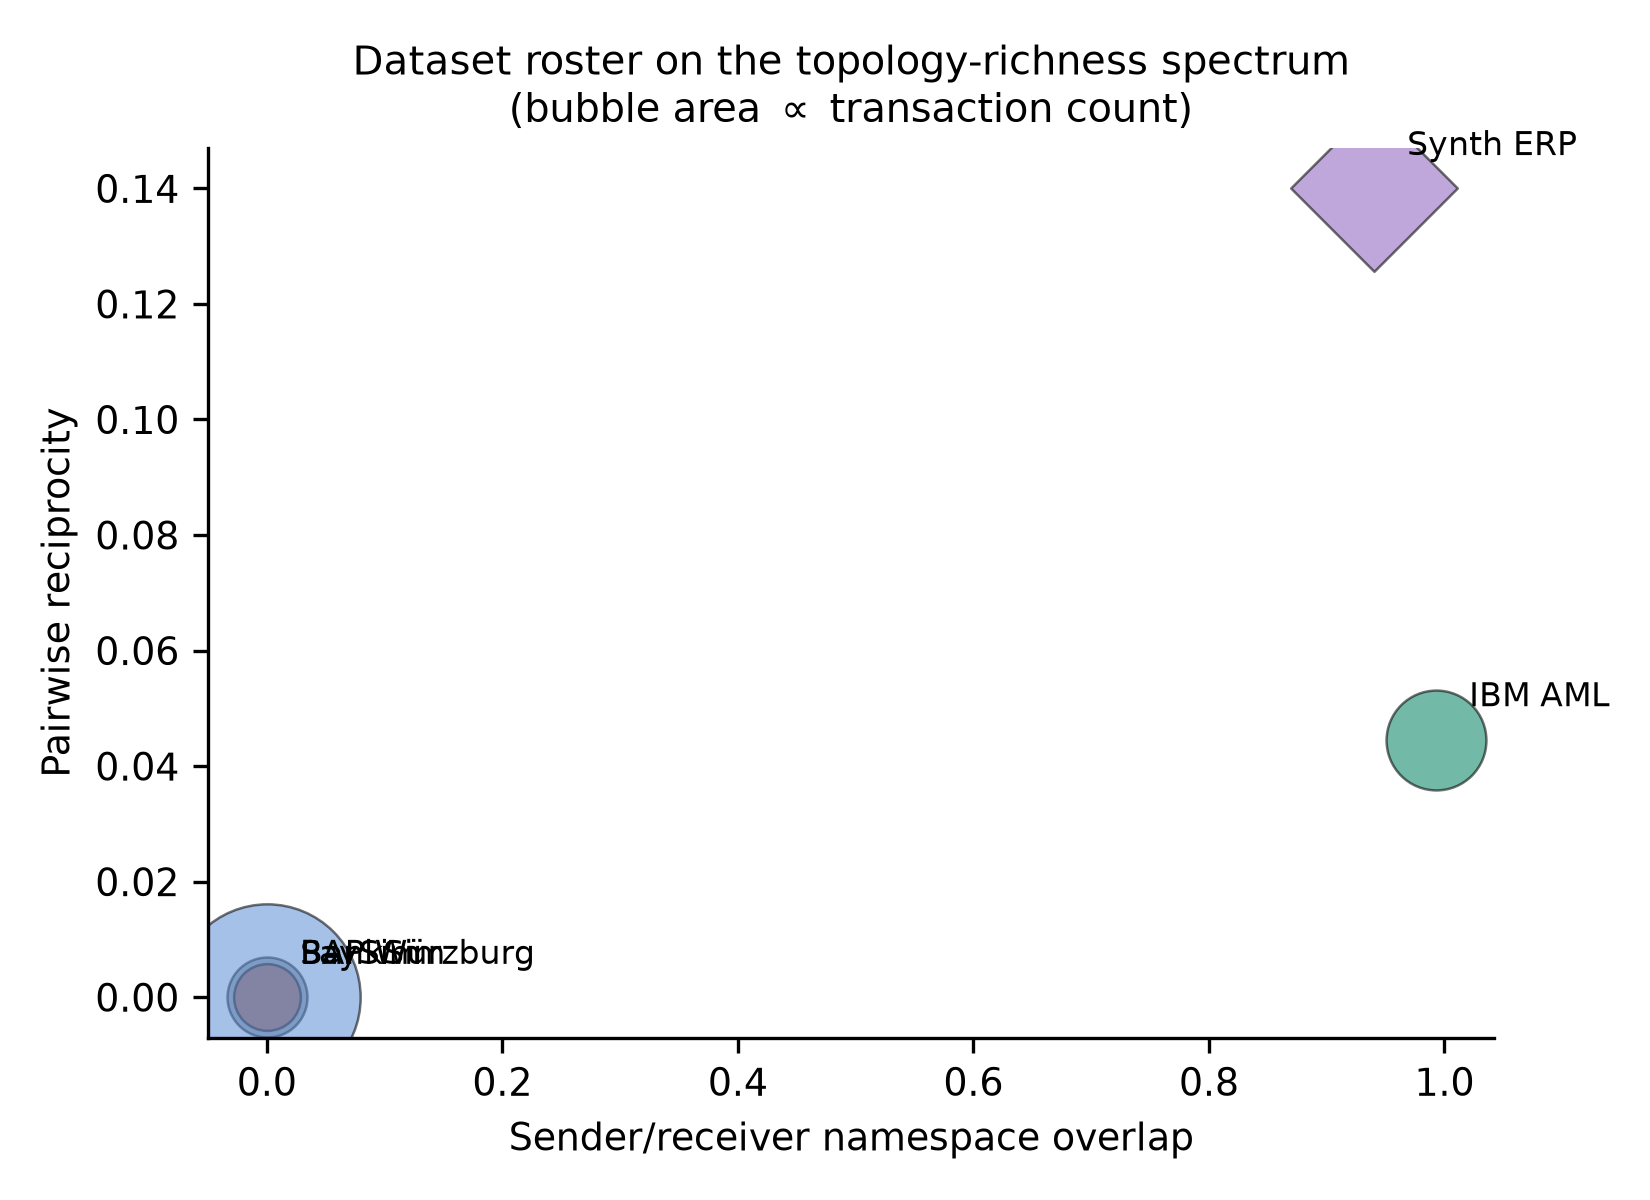
\includegraphics[width=\columnwidth]{figures/dataset_topology_spectrum.png}
  \caption{The five datasets positioned on the two structural axes this
  study uses to justify the roster: sender/receiver namespace overlap
  ($x$) and pair reciprocity ($y$), bubble area proportional to
  transaction count. IBM AML and \texttt{synth\_erp} anchor the
  structure-rich end; BankSim, SAP W\"urzburg, and PaySim anchor the
  structurally sparse end.}
  \label{fig:topology_spectrum}
\end{figure}
